\documentclass[conference]{IEEEtran}
%\documentclass[journal]{IEEEtran}
\usepackage{graphicx}
%\documentclass[]{article}

%\usepackage{draftwatermark}\SetWatermarkText{Not For Distribution}
%\SetWatermarkScale{2}\SetWatermarkLightness{0.85}

\newcommand{\ppv}{P_{pv}}
\newcommand{\pinv}{P_{inv}}


\title{System Efficiency Improvements for Standalone Grid Systems}

\begin{document}



%\abstract{}


\author{
\IEEEauthorblockN{Daniel Soto}
\IEEEauthorblockA{
The Earth Institute\\
Columbia University\\
New York, NY 10027}
\and
\IEEEauthorblockN{Vijay Modi}
\IEEEauthorblockA{
Department of Mechanical Engineering\\
Columbia, University\\
New York, NY  10027}
}

\maketitle

\begin{abstract}
Abstract.
\end{abstract}

\section{Introduction}

The cost of renewable and distributed energy systems must be
optimized to provide electricity to the customers beyond the
reach of the grid.

Communities in developing countries do not have easy access
to capital.
This constraint makes it necessary to optimize energy systems
for cost.
This work presents opportunities for efficiency and therefore
cost reduction in the areas of power conversion and storage.
These recommendations are based on data collected from customers
who have recently been provided with a near-grid-quality
electrical connection and are paying for that power on a
per kilowatt-hour basis.
There are many optimizations of system size in the literature
\cite{optimizations}.
This work adds to the literature by considering the effects
of the time of day of usage and the efficiencies of commonly
used inverters and batteries.


%We treat the hourly load profile and its effect on the
%generation and storage needed.
%We also observe for most of the systems that there is a wide variation
%in the system load with most power consumption in the evening.
%In a system that relies on an inverter, the inverter is run at a very
%inefficient operating point for much of the time.
%This lowers the overall efficiency of the system, increasing the
%necessary generation and storage costs.
%
%If the system is run inefficiently during the daytime, the inefficiency
%burden only impacts the amount of generation capacity needed.
%If the system is run inefficiently during the evening, both the
%generation and the storage costs are affected, multiplying the
%penalty.
%
%In this work we explore the interplay between consumption coincident
%with generation and consumption at different times from generation
%and quantify the impact on system costs.
%
%Two approaches to mitigation exist, the first is scheduling of loads
%to attempt to smooth consumption.
%Two of our sites have added refrigerators and we show the load duration
%curve with the addition of these devices and the effect on overall
%efficiency.
%
%The second approach is developing
%a power solution that is less sensitive to the variation in loads.
%We quantify the potential savings of each of these approaches.
%The approaches include parallel inverters, inverters with a
%standby mode, and DC distribution.
%
%
%When electricity is first delivered, use will likely be predominantly
%at nighttime.
%This means that there will be long periods of time where the power
%conversion electronics, usually inverters, are running at a low
%efficiency.
%This adds to the generation and storage burden of the system.
%
%We demonstrate this in a simple model where an assumed inverter curve
%is used and clear sky insolation is used for different daily
%loads.
%This is compared against a power conversion device with a flat
%efficiency curve.
%
%We argue for the development or adaptation of emerging technologies
%for the off-grid space.
%Some of these advanced technologies are cost competitive now.
%In this paper we describe some of the techno-economic
%details in the provision of standalone PV systems
%in rural areas.


\section{Microgrid and Data Description}
\subsection{Data collection}
We have installed 17 microgrid systems with remote connectivity
in Mali and Uganda \cite{ICTD}.
Each of these systems consists of a 1.4 kWp array of photovoltaic
panels with a 48 V, 360 Ah battery bank.
An MPPT charge controller handles battery charging and a
750 W inverter supplies the microgrid with 50 Hz, 220 V power.
Up to 20 customers are connected to these systems in a star
topology where each customer has a dedicated wire to the
central facility.
Each customer is metered by a commercially available device that
allows for energy measurement and reporting and a switch to
automatically connect or disconnect the consumer.
These systems send data on an hourly basis to a central server
using SMS messages.
Data is collected on the energy consumption of each household
as well as the AC energy consumption of the entire system.
From the solar controller, we measure and store hourly information
on the solar energy delivered to the system and the battery
voltage.

\subsection{Timeseries Description}
These messages allow us to create a database of timeseries
information from the customers.
For most customers, the peak power is consumed in the evening
as shown in Figure \ref{two-bulb-profile}.
Most of the customers have little or no usage during the day time.
The system however, uses about 50W to run the metering, computation,
and communication electronics giving a similar profile but with
a larger daytime use.

\begin{figure}[h]
\begin{center}
\includegraphics[trim = 0.0in 0.7in 0.0in 0.4in, clip, width=\columnwidth]
{figures/pchpp-ml03-217.pdf}
\end{center}
\caption{Customer exhibiting two bulb lighting load.
Each data point is the hourly load for a single day.
Multiple days are superimposed.
Points are transparent so that frequent measurements appear darker.
This customer displays two common evening power levels corresponding
to the use of one or two lightbulbs.
This not that this customer has very small power use during the day.}
\label{two-bulb-profile}
\end{figure}

We have provided two freezers that customers are using to
sell ice or frozen drinks.
The hourly profile for the household using this freezer
is shown in Figure \ref{freezer}.
These freezers draw a much larger amount of power than the
typical lighting load and have a lower variation when measured
on an hourly basis.

\begin{figure}[]
\begin{center}
\includegraphics[trim = 0.5in 0.8in 0.5in 0.9in, clip, width=\columnwidth]{figures/ml06-16.pdf}
\end{center}
\caption{Freezer load.}
\label{freezer}
\end{figure}


\subsection{Load Duration Curves}
If we sort the hourly power demand over a long time period, we
construct a curve called a load duration curve \cite{REEPS}.
A load-duration curve (Figure \ref{ldc}) shows this variation.
In the microgrid (ml07) that does not have a freezer, the most common
power level is less than 50W, which is well below the peak
efficiency of the inverter.
For the system that does have a freezer, the system spends the bulk
of its time consuming on the order of 200W, which is much closer
to the peak efficiency operating point of the inverter.
The inverter is sized so that the maximum customer load is safely
accommodated by the inverter.
However, there is a substantial efficiency penalty for operating the
inverter below the optimal point.

We can express these loads in terms of the capacity factor,
where the capacity factor is relative to the rated output
of the inverter.
Systems with high power variability will lose efficiency since
the system will often be operated outside of the range of
peak efficiency.


These systems have a 1.4 kWp solar array and an inverter rated
at 750W.

\begin{figure}[h]
\begin{center}
\includegraphics[trim = 0.0in 0.4in 0.0in 0.5in, clip, width=\columnwidth]{figures/two-ldc.pdf}
\end{center}
\caption{Load duration curve for two typical microgrid system,
including metering, computing, and computation.
Inverter and charge controller consumption is not included.
One system includes a significant daytime refrigeration load,
while the other does not.
}
\label{ldc}
\end{figure}

\subsection{Overall System Efficiency}

We can estimate an overall system efficiency from the
usage data and information from the solar controller
on photovoltaic energy generation.
This estimate of the overall efficiency of the system
is defined as power delivered by solar
power controller divided by the power delivered to the system.
We do not include the parasitic power consumed by the electronics.

Our data shows that as the capacity factor of the inverter
increases, the overall system efficiency improves.

The large variations in loads exhibited by these customers prompted
us to investigate the impact on system efficiency that these
loads are causing.
We pursued both a measurement of the systems and a simulation approach.

\begin{table}
\centering
\begin{tabular}{c c c}
Meter & System Utilization Factor & System Efficiency \\
\hline
ml03 & 0.38 & 0.62 \\
ml05 & 0.33 & 0.69 \\
ml06 (freezer) & 0.54 & 0.88 \\
ml08 (freezer) & 0.55 & 0.90 \\
\end{tabular}
\caption{System Utilization and system efficiency}
\label{efficiency}
\end{table}




In ML06, which has considerable daily load, we see an overall
efficiency of 0.89.
In ML05, with much less daily load, the overall efficiency
is 0.78.

\section{System and Simulation Description}

We examine the effect of load variation and alternate technologies
by creating a simulation of the system.
The model uses energy as the quanitity being modeled.
The simulation finds the minimum panel size and battery capacity
that will meet the demand assuming clear-sky radiation.
The model is intended to allow comparisons between systems and
load profiles rather than provide accurate guidance for system
sizes over a typical meteorological year.
The simulation takes as input the hourly load profile from a
set of customers.
In the following simulations we use both measured and simulated
loads.
Based on the hourly load profile, the energy in the battery
is simulated.
The battery is considered to be a simple energy storage device
with perfect efficiency during charging and an efficiency of
$\eta_B$ on discharge.
The panel size in the model is adjusted until the energy remaining
in the battery at the end of the simulation is equal to the
energy at the start of the simulation.
The minimum battery size is then the peak-to-peak variation
of the battery energy time series.
A time series trace is shown in Figure \ref{simulation}.

We can calculate the energy in the battery in discrete time
steps according to the following equation.
%
$$ E_B(t+\Delta t) = E_B(t)
                   + P_{charge} \cdot \Delta t
                   - \frac{P_{discharge} \cdot \Delta t}{\eta_B}
                   $$
%
Where $P_{charge}$ is the power flow when the photovoltaic
production is greater than the inverter demand and
$P_{discharge}$ is the power flow when the inverter demand
is greater than the photovoltaic power available.
They are given by the following equations.
%
$$ P_{charge} = \left\{
			  \begin{array}{rl}
			  0 & \pinv > \ppv \\
			  \ppv - \pinv & \pinv < \ppv
			  \end{array}
			  \right. $$
%
$$ P_{discharge} = \left\{
			  \begin{array}{rl}
			  \pinv - \ppv & \pinv > \ppv \\
			  0 & \pinv < \ppv
			  \end{array}
			  \right. $$
%
The power demanded by the inverter is calculated using the efficiency
of the inverter as a function of temperature according to 
$$ \pinv = \frac{P_{AC}}{\eta_{inv}(P_{AC})} $$.

\begin{itemize}
\item $E_B(t)$ the battery energy available at time $t$
\item $\ppv$ Power produced by the PV panel
\item $\pinv$ Power demanded by the inverter
\end{itemize}


\begin{figure}[h]
\begin{center}
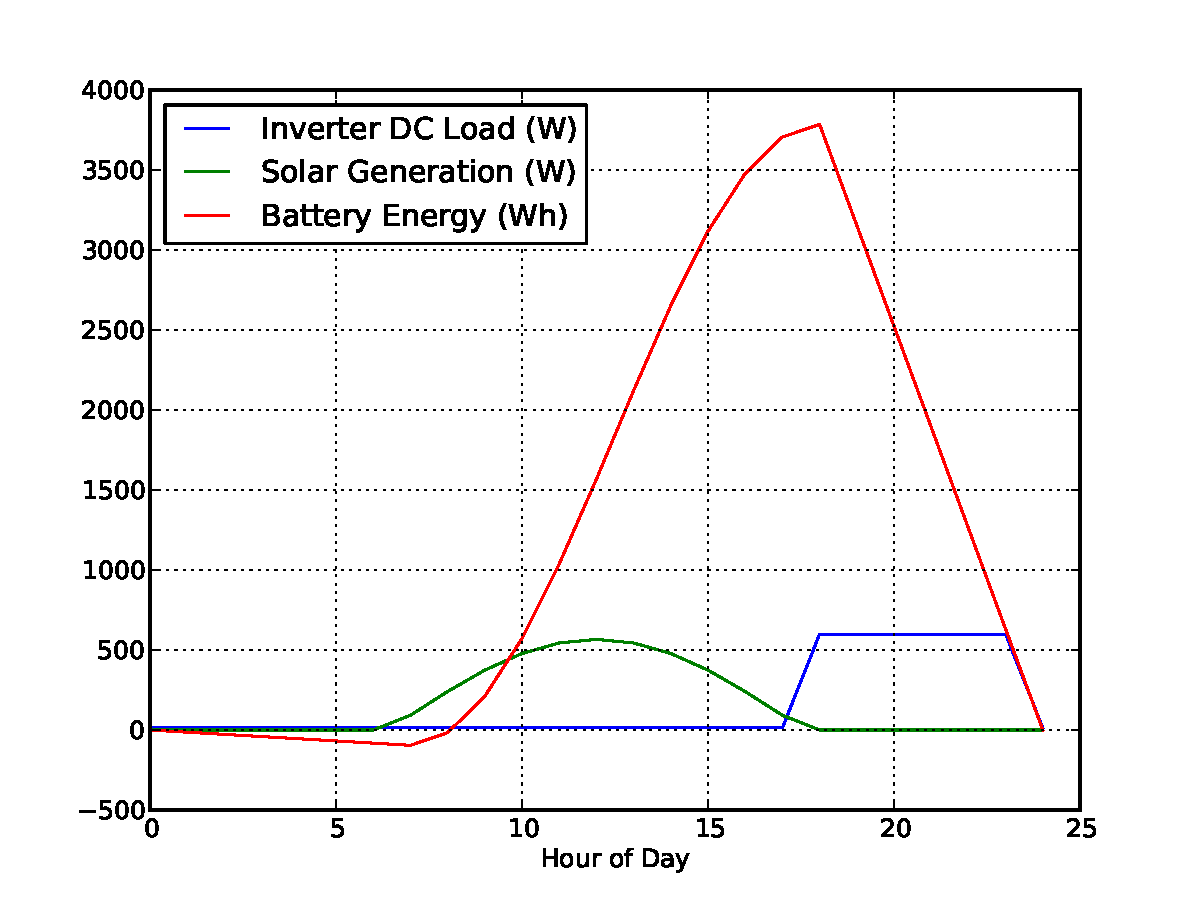
\includegraphics[trim = 0.0in 0.2in 0.0in 0.5in, clip, width=\columnwidth]{figures/simulation.pdf}
\end{center}
\caption{
Simulation.
}
\label{Graph of simulation output.}
\end{figure}

\subsection{Baseline System}
The simulated baseline system is based on the system we have
installed in the field.
The inverter efficiencies for this system are shown in Figure
\ref{inverter_curves}.

\begin{figure}[]
\begin{center}
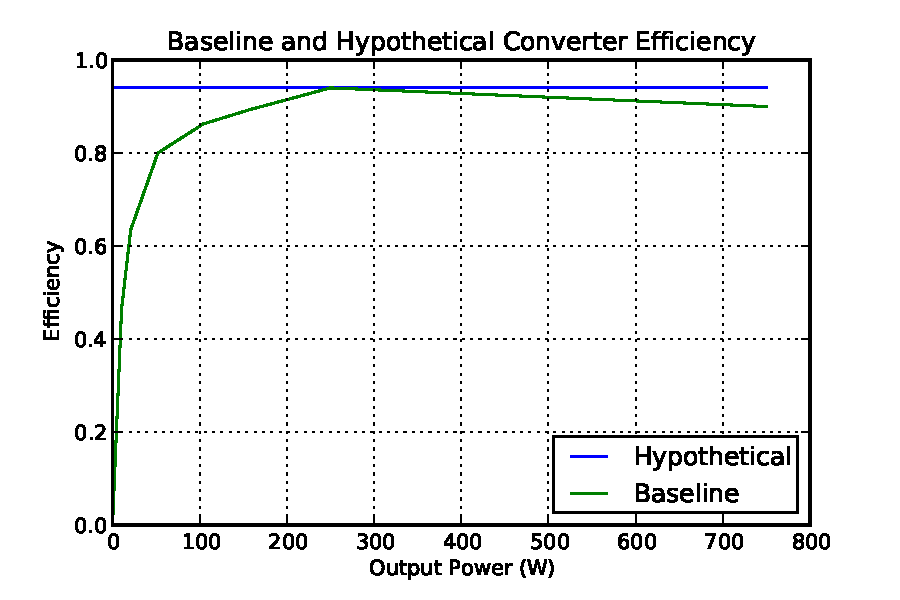
\includegraphics[width=\columnwidth]{figures/inverter_curves.pdf}
\end{center}
\caption{Efficiency curves for baseline and proposed system.}
\label{inverter_curves}
\end{figure}

\section{Simulation Results}

We compare the results of a baseline system with a typical
inverter and lead acid battery to a system using an
power conversion device with flat efficiency curve.

\subsection{Impact of load variation and time on system size}

During the day, current and power flows directly from the output of
the charge controller, through the inverter to the load.

We look at three loads that take 1 kWh per day.
The first load is
evenly distributed throughout the day, the second load is
consumed in 6 hours after solar production has ceased, and the third
load is centered around solar noon.

For each of these loads, we calculate the minimum necessary generation
and storage to satisfy the load.
This calculation will take into effect the efficiency losses in
the inverter and the battery.

For these three cases, the generation capacity changes slightly
to reflect the system efficiencies.

The daytime and nighttime load are hypothetical 1800 Wh loads over a
6 hour period.

Table \ref{load_type_impact}, shows the results of simulations
which demonstrate the variability of panel size and battery
size with the type of load.
Each of these loads have the same daily energy total but
occur at different times of day.
This causes about a 10\% variation in panel area and a
nearly three-fold change in the minimum battery size needed.

\begin{table}
\centering
\begin{tabular}{c c c}
Configuration & Panel          & Minimum Battery \\
              & Area (m$^2$)   & Size (kWh)      \\
\hline
Baseline System, Daytime Load   & 2.83 & 0.76 \\
Baseline System, Nighttime Load & 2.94 & 3.88 \\
Baseline System, Constant Load  & 3.05 & 2.46 \\
Baseline System, Village Load   & 3.08 & 2.93 \\
\end{tabular}
\caption{Impact of type of load on system size.
Loads are normalized to 3.0 kWh per day.}
\label{load_type_impact}
\end{table}


\begin{table}
\centering
\begin{tabular}{c c c}
Configuration & Panel          & Minimum Battery \\
              & Area (m$^2$)   & Size (kWh)      \\
\hline
Typical Inverter, Daytime Load   & 2.3 & 0.4 \\
Typical Inverter, Nighttime Load & 2.9 & 3.3 \\
Typical Inverter, Constant Load  & 2.6 & 2.0 \\
Flat Inverter, Daytime Load      & 1.7 & 0.5 \\
Flat Inverter, Nighttime Load    & 2.1 & 2.6 \\
Flat Inverter, Constant Load     & 1.8 & 1.4 \\
\end{tabular}
\caption{Impact of inverter non-ideality on system size}
\label{sizetable}
\end{table}

For the two types of inverters, the reduction in panel area
ranges from 27\% to 29\% when using an ideal inverter.
The impact on battery size can be positive for a daytime
load but was 21\% for a nighttime load and 30\% for a
continuous load.

\subsection{Battery Chemistry}

Lead acid batteries have round trip energy efficiencies on the
order of 75\%.
Lithium-ion chemistry batteries demonstrate better round trip
efficiencies.
These efficiencies impact both the storage needs of the system
and the generation needs of the system.

Results for 95\% efficient battery (compare to baseline).

\begin{table}
\centering
\begin{tabular}{@{} p{0.5\columnwidth}
                @{} c
                @{} c @{}}
Configuration & Panel          & Minimum Battery \\
              & Area (m$^2$)   & Size (kWh)      \\
\hline
Typical Inverter, 95\% Batt, Daytime Load   & 2.2 & 0.4 \\
Typical Inverter, 95\% Batt, Nighttime Load & 2.3 & 2.6 \\
Typical Inverter, 95\% Batt, Constant Load  & 2.2 & 1.6 \\
Typical Inverter, 95\% Batt, Village Load   & 2.5 & 3.4 \\
\end{tabular}
\caption{Impact of inverter non-ideality on system size}
\label{sizetable}
\end{table}


While lithium batteries are a factor of XX more expensive
than lead-acid batteries based on the capacity of the battery
(USD/kWh), the cost per delivered watt-hour of electricity
over the lifetime of the battery is comparable.
Additional economic improvement is gained by lower weight
for shipping and improved round trip efficiency which lowers
both the battery capacity and the generation capacity when nighttime
loads are needed.

\section{Discussion}
Here we discuss what methods are available to mitigate the
load variations and increase efficiencies.

\subsection{Mitigating Load Variation}
Systems with better no-load performance should be used to counteract
the problem of efficiency at the lower end.

Two solutions exist for this problem, the first is to remove
the constant loads (meter electronics, communication, and
computing) from the inverter.
This could allow an inverter to operate in a power-down or
search mode for most of the time and then switch on only
to service loads.

\subsubsection{Slaved inverters}
A chain of inverters that turn on in a cascaded fashion could
be more efficient.

\subsubsection{Inverters with Standby Mode}
The standby loss could be low but an small use will energize the
entire system.

\subsubsection{DC Distribution}
If the efficiency curve of a DC/DC converter were favorable,
a high-voltage direct current (HVDC) distribution scheme could
be used.
Our testing of a 48 VDC to 12 VDC converter is over 80\% for
the range of power of interest.
The no-load dissipation for this device was below our measurement
capacity of 0.5W.


\subsection{Battery Chemistry}

\subsection{Distributed Storage}
Another possibility is local storage at the home with a small inverter
that the customer only switches on during times when power
is needed.
This reduces the standby load to zero but likely adds to the
fixed cost of the system.

\subsection{Load Duration Curve}



What is the impact of this inefficiency on battery life?

We can simulate the effective inverter efficiency for a given
load profile and inverter curve.

$$ \eta_{effective} = \frac{\sum P_{AC} \cdot \Delta t}
                          {\sum P_{AC} /\eta_{inv} \cdot \Delta t} $$




\subsection{Using Real vs Apparent Power}
Almost all loads used by customers in our microgrids have power
factors below one.
These switching power supplies negatively affect inverter efficiency
and thus the battery supply.
To properly account for the customer wear and tear on the battery
it likely makes more sense to charge for apparent power or for
real power adjusted by power factor.







\section{Summary}
Hourly demand data for newly electificed communities has been gathered.
We find that improving no-load and low load power consumption of the
inverter can reduce storage and generation needs.

\begin{thebibliography}{1}
\bibitem{optimizations}
Z Wissem, K Gueorgui, K H\'edi,
Modeling and techinical--economic optimization of an autonomous
photovoltaic system,
Energy, Vol. 37, 2012 pp. 263-272
(doi:10.1016/j.energy.2011.11.036)
\bibitem{ICTD}
D.~Soto, SharedSolar. ICTD 2012.
\bibitem{REEPS}
G.~Masters,
"Renewable and Efficient Electric Power Systems",
Wiley Interscience,
2004
\end{thebibliography}


\end{document}

%---------------------------------------------------------------------------%
%---------------------------------------------------------------------------%
%---------------------------------------------------------------------------%
%---------------------------------------------------------------------------%
%---------------------------------------------------------------------------%
%---------------------------------------------------------------------------%
%---------------------------------------------------------------------------%
%---------------------------------------------------------------------------%
%---------------------------------------------------------------------------%
%---------------------------------------------------------------------------%
%---------------------------------------------------------------------------%
%---------------------------------------------------------------------------%



We have measured the load patterns of users and have generated
load-duration curves over a N-day period.
From this curve, (Figure \ref{ldc}) we estimate the overall
efficiency of the inverter.
$$ \sum p_i / \eta_i $$
The overall inverter efficiency is much lower than its rated
efficiency because the inverter is operated for so much time
at a low fraction of its capacity.


%$$ \ppv = insolation \cdot array size \cdot array efficiency
%         \cdot controller efficiency $$

